\section{Grundbegriffe}

\begin{df}\label{1.1}
Eine nicht-leere Menge $G$ mit einer Verknüpfung $\ast$
heißt \textbf{\textit{Gruppe}}, falls
\begin{enumerate}
\item[\textbf{(i)}]
$\forall g,h,k \in G: \ (g \ast h) \ast k = g \ast (h \ast k) \ \quad  \quad \quad \quad \quad \quad \quad
  (\textit{assoziativ}) $   
\item[\textbf{(ii)}] 
$\exists ! e \in G \ \forall g \in G: \ g \ast e = e \ast g  = g  \  \quad  \quad \quad \quad \quad \quad \quad \quad \quad  (\textit{neutrales Element}) $   
\item[\textbf{(iii)}]
$\forall g \in G \ \exists ! g^{-1} \in G: \ g \ast g^{-1} = g^{-1} \ast g = e \ \  \quad \quad \quad \quad \quad \quad (\textit{inverses Element})$  
\end{enumerate}
erfüllt sind. Man schreibt dann auch $(G,\ast)$.
\index{Gruppe}
\end{df}



\begin{generic_no_num}{Bemerkungen}
\ 
\begin{enumerate}
\item[\textbf{(1)}]
Die Axiome $\textbf{(ii)}$ und $\textbf{(iii)}$ lassen sich mit
\begin{enumerate}
\item[$ \textbf{(ii)}^\prime $]
$\exists e \in G \ \forall g \in G : \ e \ast g = g$
\item[$ \textbf{(iii)}^\prime $]
$\forall g \in G  \ \exists h \in G : \ g \ast h = e$
\end{enumerate}
abschwächen und herleiten.
\item[\textbf{(2)}]
\textit{(Rechenregeln einer Gruppe)}
\begin{enumerate}
\item[ \textbf{(i)}]
$g  \ast x = g \ast y  \Rightarrow x = y  \qquad \qquad \ \textit{(Kürzungsregel)}$
\item[ \textbf{(ii)}]
$\forall g \in G : \ (g^{-1})^{-1} = g $
\item[\textbf{(iii)}]
$g \ast g = g \Rightarrow g = e  \qquad \qquad \qquad \textit{($e$ ist als einziges Element idempotent)}$
\item[\textbf{(iv)}]
$(g \ast h)^{-1} = h^{-1} \ast g^{-1}$
\item[\textbf{(v)}]
$\forall a,b \in G \ \exists ! x \in G : \ a \ast x = b$
\end{enumerate}
\item[\textbf{(3)}]
Eine Verknüpfung $\ast$ ist eine Abbildung der Form	$G \times G \to G , \ (g,h) \mapsto g \ast h$.
\end{enumerate}

\end{generic_no_num}

\begin{df}
Eine Gruppe $(G,\ast) $ mit $g \ast h = h \ast g$ für alle $g,h \in G$
heißt \textbf{\textit{kommutativ}} oder \textbf{\textit{abelsch}}.
\index{Gruppe!abelsch}
\end{df}

\begin{genericdf}{Beispiele}\label{1.3}\ 
\begin{enumerate}
\item[\textbf{(1)}]
Sei $X$ eine nicht-leere Menge und $\Sym(X) := \lbrace f : X \to X \ | \ f \ \text{ist bijektiv} \rbrace$.
$\Sym(X)$ bildet mit der Komposition von Abbildungen die \textbf{\textit{symmetrische Gruppe}} auf $X$.
Falls $X = \lbrace 1,...,n \rbrace$ ist, definieren wir die \textbf{\textit{symmetrische Gruppe vom Grad $n$}} durch
$S_n := \Sym(X)$ und es gilt $|S_n| = n!$.
\item[\textbf{(2)}]
$(\mathbb{Z},+)$, $(\mathbb{Q}^\ast,\cdot)$ und $O(n,\mathbb{R})$ sind Gruppen. Mit $\Q^\ast$ ist hier $\Q \setminus \lbrace 0 \rbrace$ gemeint.
\end{enumerate}
\index{Gruppe!symmetrisch}
\end{genericdf}

\begin{df}\label{1.4}
Sei $G$ eine Gruppe.
$U \subseteq G$ heißt \textbf{\textit{Untergruppe}}, falls
\begin{enumerate}
\item[\textbf{(i)}]
$1_G \in G$ 
\item[\textbf{(ii)}]
$\forall u,v \in U : \ u \cdot v \in U$
\item[\textbf{(iii)}]
$\forall u \in U: \ u^{-1} \in U $
\end{enumerate}
erfüllt sind.
Wir schreiben dann $U \leq G$.
\index{Untergruppe}
\end{df}

\begin{generic_no_num}{Bemerkungen} \

\begin{enumerate}
\item[\textbf{(1)}]
Sei $G$ eine Gruppe und $A,B \subseteq G$.
Dann definieren wir $A^{-1} := \lbrace a^{-1} \ | \ a \in A\rbrace$
und \\ 
$A \cdot B := \lbrace a \cdot b \ | \ a \in A \wedge b \in B \rbrace$.
Hierbei bezeichnen wir $A \cdot B$ auch als \textbf{\textit{Komplexprodukt}}. 

\item[\textbf{(2)}]
$U \subseteq G$ ist eine Untergruppe \textbf{genau dann}, \textbf{wenn}
$1_G \in U$, $U \cdot U \subseteq U$ und $ U^{-1} \subseteq U$. 

\item[\textbf{(3)}]
Sei $\lbrace U_i \rbrace_{i \in I}$ eine Familie von Untergruppen einer Gruppe $G$ und 
$I$ eine beliebige Indexmenge.
Dann gilt $\bigcap_{i \in I} U_i \leq G$.
\begin{proof}
\begin{align*}
x \in \bigcap_{i \in I} U_i \Rightarrow 
\forall i \in I : \ x \in U_i \stackrel{U_i \leq G}{\Rightarrow }
\forall i \in I : \ x^{-1} \in U_i \Rightarrow
x^{-1} \in \bigcap_{i \in I} U_i
\end{align*}
Die anderen Eigenschaften aus \ref{1.4} folgen durch analoges Vorgehen.
\end{proof}

\item[\textbf{(4)}]
\textbf{\textit{Untergruppenkriterium:}} \index{Untergruppe!Kriterium}
Sei $G$ eine Gruppe. Dann gilt
\begin{align*}
\emptyset \neq U \subseteq G \ \text{Untergruppe} 
\Leftrightarrow
\forall u,v \in U : \ u \cdot v^{-1} \in U.
\end{align*}
Falls $G$ endlich ist gilt sogar
\begin{align*}
\emptyset \neq U \subseteq G \ \text{Untergruppe} 
\Leftrightarrow
\forall u,v \in U : \ u \cdot v \in U.
\end{align*}
\end{enumerate}
\end{generic_no_num}

\begin{genericdf}{Beispiel}
$\Sl_n(K) := \lbrace A \in \Gl_n(K) \ | \det(A) = 1   \rbrace \leq \Gl_n(K)$
\end{genericdf}

\begin{df} \label{1.6}
Sei $G$ eine Gruppe und $S \subseteq G$.
Dann ist 
\begin{align*}
<S> := \bigcap \limits_{U_i \leq G, S \subseteq U_i} U_i
\end{align*}
das \textbf{\textit{Erzeugnis von $S$}}.\index{Erzeugnis}
\begin{enumerate}
\item[\textbf{(1)}]
$<S>$ ist die kleinste Untergruppe von $G$, die $S$ enthält.
Gilt $S = \lbrace g \rbrace$ für $g \in G$, dann schreiben wir $<g>$ anstatt $<S>$.
Wir nennen dies die von \textbf{\textit{$g$ erzeugte zyklische Untergruppe von $G$}}.\index{Untergruppe!zyklische}
Falls ein $g \in G$ existiert mit $G = < g>$, nennen wir $G$ \textbf{\textit{zyklisch}}.\index{Gruppe!zyklisch}  
\item[\textbf{(2)}]
Falls $S = \emptyset$ ist, gilt $<S> = \lbrace 1_G \rbrace =: 1$.
\end{enumerate}
\end{df}

\begin{genericthm}{Lemma}\label{1.7}
Sei $G$ eine Gruppe und $\emptyset \neq S \subseteq G$.
Dann gilt
\begin{align*}
<S> = \lbrace s_1 \cdot s_2 \cdots s_r \ | \ r \in \mathbb{N}, \ s_i \in S \cup S^{-1} \rbrace
\end{align*}
und für $S= \lbrace g \rbrace $ somit $<g> = \lbrace g^m \ | \ m \in \mathbb{Z} \rbrace$. \\
Hier fließt die Konvention $g^0 = 1_G$ und $g^{-k} = (g^{-1})^k$ für $k \in \mathbb{N}$ ein.
\end{genericthm}

\begin{proof}
Sei $H = \lbrace s_1 \cdot s_2 \cdots s_r \ | \ r \in \mathbb{N}, \ s_i \in S \cup S^{-1} \rbrace$.
Zunächst zeigen wir die Hinrichtung.
Wegen $1_G = s \cdot s^{-1}$ für beliebiges $s \in S$ gilt $1_G \in H$.
Durch schnelles Nachprüfen sind auch Produkte und Inverse von $H$ in $H$.
Also folgt $H \leq G$, $S \subseteq H$ und mit \ref{1.6} gilt $<S> \subseteq H$.
Für die Rückrichtung sei $U \leq G$ mit $S \subseteq U$.
Damit gilt $H \subseteq U$ und 
\begin{align*}
<S> = \bigcap \limits_{U \leq G, S \subseteq U} U
\Rightarrow 
H \subseteq <S>.
\end{align*}
Damit sind wir fertig.
\end{proof} 

\begin{genericthm}{Lemma}\label{1.8}
Sei $G = <g>$ mit $|G| = d$.
Dann gilt $G = \lbrace 1_G, g ,g^2,...,g^{d-1} \rbrace$
und \\ 
$d = \min\lbrace i \in \mathbb{N} \ | \ g^i = 1_G \rbrace$.
Für $k \in \mathbb{Z}$ mit $g^k = 1_G$ gilt $d | k$.
\end{genericthm}

\begin{proof}
Nach \ref{1.7} ist $G = \lbrace g^m \ | \ m \in \mathbb{Z} \rbrace$.
Aufgrund der Endlichkeit von $G$ existieren $i$ und $j$ 
mit $i > j > 0$ und $g^i = g^j$. Also folgt
\begin{align*}
g^{i-j} = g^j \cdot g^{-j} = 1_G, \quad i-j \in \mathbb{N},
\end{align*}
womit ein minimales $d^\prime \in \mathbb{N}$ mit $g^{d^\prime} = 1_G$ existieren muss. 
Nun wählen wir $k \in \mathbb{Z}$ beliebig, aber fest.
Dann existieren $q \in \mathbb{Z}$ und $0 \leq r \leq d^{\prime} $, sodass 
$k = q \cdot d^{\prime} + r$ gilt.
Damit folgt
\begin{align*}
g^k = g^{q \cdot d^{\prime} + r} = g^{q \cdot d^{\prime}} \cdot g^r
= \left( g^{d^{\prime}} \right)^q \cdot g^r = g^r
\end{align*}
und somit $<g> = \lbrace 1_G, g ,g^2,...,g^{d^\prime-1} \rbrace$.
Für $g^k = 1_G$ muss dann $g^r = 1_G$ gelten. 
In diesem Fall erhalten wir aufgrund der Minimalität von $d^\prime$, dass 
$r = 0 $ ist. Also gilt $ k = q \cdot d^\prime$ und somit $d^\prime | k$.
Wäre $g^i = g^j$ für $d^\prime \geq j > i >0$, würde
$g^{j-i} = 1_G$ für $1 \leq j-i < r$ folgen.
Dies ist ein Widerspruch zur Minimalität von $d^\prime$.
Insgesamt folgt also $d = d^\prime$.
\end{proof}

\begin{df}\label{1.9}\index{Ordnung!Gruppe}\index{Ordnung!Element}
Sei $G$ eine Gruppe. Die Kardinalität $|G|$ bezeichnet man als \textit{Ordnung von $G$}.
Für $g \in G$ nennen wir $|<g>|$ die \textbf{\textit{Ordnung des Elements $g$}} und schreiben hierfür $o(g)$.
\begin{enumerate}
\item[\textbf{(1)}]
Falls $G$ endlich ist, beschreibt $|G|$ die Anzahl der Elemente.
\item[\textbf{(2)}]
An $(\mathbb{R},+)$ sehen wir, dass $|G|$ überabzählbar sein kann.
\item[\textbf{(3)}]
Die Ordnung eines Elements $o(g)$ kann endlich oder abzählbar unendlich sein.
Im zweiten Fall schreiben wir $o(g) = \infty$.
\end{enumerate}
\end{df}

\begin{genericdf}{Beispiel}
\index{Permutation}
Sei $G = S_n$ die symmetrische Gruppe vom Grad $n$.
Ein Element $\pi \in S_n$ nennen wir \textit{Permutation}.
Durch
\begin{align*}
 \pi = \bigl(\begin{smallmatrix}
    1 & 2 & 3 & \cdots & n-1 & n \\
    \pi(1) & \pi(2) & \pi(3) & \cdots &  \pi(n-1)  & \pi(n)
  \end{smallmatrix}\bigr)
\end{align*}
können wir $\pi$ als Abbildung beschreiben. Jedoch ist dies ziemlich umständlich.
Um dies zu umgehen führen wir die \textbf{\textit{Zykelschreibweise}} ein.\index{Permutation!Zykelschreibweise}
\begin{figure}[H]
  \centering
    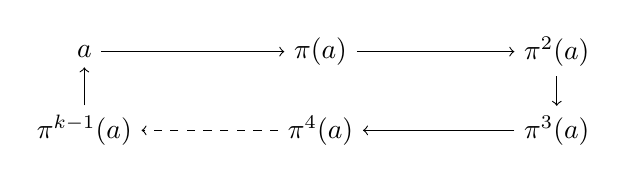
\begin{tikzpicture}
		\node (A) at (0,0)  {$a$};
		\node (B) at (3,0) {$\pi(a)$};
		\node (C) at (6,0) {$\pi^2(a)$};
		\node (D) at (6,-1) {$\pi^3(a)$};
		\node (E) at (3,-1) {$\pi^4(a)$};
		\node (F) at (0,-1) {$\pi^{k-1}(a)$};
		\draw[->] (A) to (B);
		\draw[->] (B) to (C);
		\draw[->] (C) to (D);
		\draw[->] (D) to (E);
		\draw[->,dashed] (E) to (F);
		\draw[->] (F) to (A);
\end{tikzpicture}
\caption{Zykel}
\end{figure}
Für ein $a \in \lbrace 1,...,n \rbrace$ ist $(a , \pi(a), \pi^2(a),...,\pi^{k-1}(a) )$ ein Zykel in $\pi$.
Hierbei setzen wir \\ 
$k := \min\lbrace i \in \mathbb{N}_0 \ | \ \pi^k(a) = a \rbrace$. Deswegen kommt eine Ziffer in einem Zykel auch nur ein einmal vor.
Mit den Äquivalenzklassen der Relation 
\begin{align*}
i \sim j \Leftrightarrow  \exists l \in \mathbb{N} : \pi(i)^l = j
\end{align*}
erhalten wir die verschiedenen Zykel bezüglich $\pi$.
Wir betrachten nun 
\begin{align*}
\pi = \bigl(\begin{smallmatrix}
    1 & 2 & 3 & 4 & 5  \\
    3 & 5 & 4 & 1 &  2  
  \end{smallmatrix}\bigr)
\end{align*}
aus $S_5$. In dieser Permutation sind die Zykel
\begin{figure}[H]
  \centering
    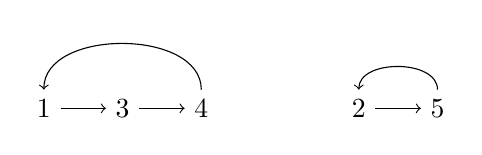
\begin{tikzpicture}
		\node (A) at (0,0)  {$1$};
		\node (B) at (4,0) {$2$};
		\node (C) at (1,0) {$3$};
		\node (D) at (2,0) {$4$};
		\node (E) at (5,0) {$5$};
		
		\draw[->] (A) to (C);
		\draw[->] (B) to (E);
		\draw[->] (C) to (D);
		\draw[->,out=90, in=90] (D) to (A);
		\draw[->,out=90, in=90] (E) to (B);
\end{tikzpicture}
\end{figure}
enthalten. Wir lassen die Zykel der Länge $1$ weg, wenn klar ist, in welchem $S_n$ gerechnet wird.
Nun betrachten wir noch ein konkretes Beispiel aus der $S_3$.
In $S_3$ sind $(1 2),(1 3), (2 3), (1 2 3),$ $(1 3 2)$ und $\id$ enthalten.
Es sind also fünf Untergruppen, die von einem Element erzeugt werden. Die zyklischen Untergruppen sind
$<(1 2)>, <(1 3)>, <(2 3)>, <(1 2 3)>$ und $< \id >$.
%\textcolor{red}{\textbf{Sind es wirklich 6? $(1 3 2)$ ist nämlich in $<(1 2 3)>$ enthalten. }}
\end{genericdf}

\begin{genericdf}{Beispiel}\label{1.11}
Sei $G = ( \mathbb{Z}, + )$. Nun fragen wir uns, wie die Untergruppen von $G$ aussehen.
Für $m \in \mathbb{N}_0$ sind $m  \mathbb{Z} = \lbrace z \in \mathbb{Z} \ | \ z = m \cdot x, \ x \in \mathbb{Z} \rbrace = < m >$  Untergruppen von $\mathbb{Z}$.
Aber haben alle Untergruppen von $\mathbb{Z}$ diese Form? Wir können diese Frage mit ja beantworten.
\begin{proof}
Sei $U \leq Z$ eine beliebige Untergruppe. Interessant wird es wenn $U \neq \lbrace 0 \rbrace $ ist.
Zunächst wissen wir, falls $ a \in U \setminus \lbrace 0 \rbrace$ ist auch $ -a \in U \setminus \lbrace 0 \rbrace$.
Da $\mathbb{Z}$ netterweise geordnet ist, finden wir auch $m := \min \lbrace a \in \mathbb{U} \ | \ a \in \mathbb{N} \rbrace$. Damit folgt $m \cdot n \in U$ für alle $n \in \mathbb{Z}$.
Damit wissen wir schon mal, dass $m  \mathbb{Z} \subseteq U$ gilt.
Sei $n \in U$ beliebig. Dann gilt $n = q \cdot m + r$ für $q,r \in \mathbb{Z}$ mit $0 \leq r < m$.
Aufgrund der Minimalität von $m$ folgt mit $r = n -q \cdot m \in U$, dass $r = 0$ sein muss. Also erhalten wir $n = q \cdot m \in m\mathbb{Z}$.
\end{proof}

\end{genericdf}

\begin{df}\label{1.12}\index{Linksnebenklassen}\index{Untergruppe!Nebenklassen} \index{Index}
Sei $G$ eine Gruppe und $U \leq G$. Mit 
\begin{align*}
g \sim h \Leftrightarrow \ \exists u \in U: \ g \cdot u = h
\end{align*}
für $g,h \in G$ erhalten wir eine Äquivalenzrelation auf $G$.
Deren Äquivalenzklassen bezeichnen wir als \textit{\textbf{Linksnebenklassen}} von $U$ in $G$.
Falls deren Anzahl endlich ist, nennen wir diese den \textit{\textbf{Index}} von $U$ in $G$ und schreiben hierfür auch $[G:U].$
Die Nebenklassen haben die Form
\begin{align*}
gU := \lbrace g\cdot u \ | \ u \in U \rbrace,
\end{align*}
wobei $g$ der Repräsentant von $gU$ ist.
\end{df}

\begin{genericdf}{Bemerkungen}\label{1.13} \ 
\begin{enumerate}
\item[\textbf{(1)}] \index{Rechtsnebenklassen}
Wir definieren analog durch
\begin{align*}
g \sim h \Leftrightarrow \ \exists u \in U: \ g = u \cdot h, \ Ug = \lbrace u \cdot g \ | \ u \in U \rbrace
\end{align*}
die \textbf{\textit{Rechtsnebenklassen}}.
Wichtig ist, dass im Allgemeinen $gU \neq Ug$ gilt.
Um dies zu verdeutlichen betrachten wir $G = S_3$ mit $U= <(12)> = \lbrace \id, (12)\rbrace $.
Mit 
\begin{align*}
(23)U &= \lbrace (23),(123) \rbrace \\
U(23) &= \lbrace(23),(132) \rbrace 
\end{align*}
folgt $(23)U  \neq U(23)$.
\item[\textbf{(2)}]\index{Normalteiler} \index{Untergruppe!Normalteiler} \index{normal}
Wir bezeichnen $U \leq G$ als \textbf{\textit{Normalteiler}} bzw. als \textbf{\textit{normal}} in $G$, falls
\begin{align*}
\forall g \in G: \ gU = Ug
\end{align*}
gilt und schreiben hierfür $ U \nt G$.
Sollte $G$ abelsch sein, sind alle Untergruppen von $G$ Normalteiler.
Mit \index{Zentrum}
\begin{align*}
Z(G) := \lbrace g \in G \ | \ \forall x \in G: \ g\cdot x = x \cdot g \rbrace \nt G
\end{align*}
bezeichnen wir das \textit{\textbf{Zentrum}} von $G$.
\end{enumerate}
\end{genericdf}

\begin{genericthm}{Satz von Lagrange}\label{1.14} \index{Satz!Lagrange}
Sei $G$ eine endliche Gruppe mit $U \leq G$. Dann wird $|G|$ von $|U|$ geteilt.
Dies bedeutet, dass
\begin{align*}
|G| =|U| \cdot |G  	/ U | = |U| \cdot |U  	\backslash  G |
\end{align*}
gilt. Mit $G  	/  U$ bezeichnen wir die Menge der Linksnebenklassen und mit
$U  	\backslash  G$ die der Rechtsnebenklassen.
Für eine beliebige Gruppe $G$ stehen alle Nebenklassen von $U$, unabhängig ob rechts- oder links, in Bijektion zu $U$. 
\end{genericthm}

\begin{proof}
Zunächst wählen wir $g \in G$ beliebig aber fest und zeigen, dass 
\begin{align*}
\varphi : U \to gU, \ u \mapsto gu
\end{align*}
bijektiv ist.
\begin{itemize}
\item $\varphi$ ist surjektiv: Sei $x \in gU$, dann existiert ein $u_1 \in U$ mit $x = g \cdot u_1$.
Damit gilt $\varphi(u_1) = x$ und $\varphi$ ist surjektiv.
\item $\varphi$ ist injektiv: Aus $\varphi(u_1) = \varphi(u_2)$ folgt $g \cdot u_1 = g \cdot u_2 $.
Weiter erhalten wir mit 
\begin{align*}
u_1 = g^{-1} \cdot (g \cdot u_1) = g^{-1} \cdot (g \cdot u_2) = u_2
\end{align*}
die Injektivität von $\varphi$.
\end{itemize}
Nun ist $G$ eine disjunkte Vereinigung seiner Linksnebenklassen.
Da $G$ endlich ist, gibt es auch nur endlich viele Repräsentanten, wir setzen hierfür $m := | G / U |$ und 
betrachten die Repräsentanten $\lbrace g_1,...,g_m \rbrace$.
Wir wissen also 
\begin{align*}
G = g_1U \cup ... \cup g_mU
\end{align*}
und mit der Bijektivität von $\varphi$ gilt 
\begin{align*}
|G| = |g_1U |+ ... + |g_mU| = m \cdot |U|.
\end{align*}
Damit haben wir die Aussage für die Linksnebenklassen gezeigt, dass Vorgehen für die Rechtsnebenklassen ist vollkommen analog.
\end{proof}

\begin{genericdf}{Beispiele und Anwendungen}\label{1.15} \
\begin{enumerate}
\item[\textbf{(1)}]
Sei $G$ eine Gruppe mit $|G| = p$ prim.
Mit \ref{1.14} haben alle Untergruppen die Ordnung $1$ oder $p$, wodurch
nur $G$ und $1$ Untergruppen sein können.
Außerdem ist $G$ zyklisch mit $G =<g>$ für $g \neq 1_G$.
Falls die zugehörige Verknüpfung additiv ist, schreiben wir $\Zn{p}$.
Falls diese multiplikativ ist, schreiben wir $C_p$.
\item[\textbf{(2)}]
Sei $G = S_3$. Wegen $|G| = 2 \cdot 3$ erhalten wir mit
\begin{align*}
1, <(12)>, <(13)>, <(23)>, <(123)>, S_3
\end{align*}
alle Untergruppen von $S_3$.
Also haben alle echten Untergruppen die Ordnung $1$, $2$ oder $3$.
In der \textbf{(1)} haben wir gesehen, dass diese dann zyklisch sind.
\item[\textbf{(3)}]
Existiert auch eine Umkehrung des Satzes von Lagrange? 
Diese können wir so formulieren:
Sei $G$ eine Gruppe mit $|G| = n$ und $d | n$.
Gibt es eine Untergruppe $U$ mit $|U| = d$?
Wir können diese Frage mit ja beantworten, wenn $G$ zyklisch ist.
\begin{proof}
Sei $G = <g>$ und $|G| = n$. Wegen $d | n $ existiert ein $k \in N$ mit $n = k \cdot d$.
Wir betrachten $g^k \in G$ mit $<g^k> \leq G$. Durch
\begin{align*}
(g^k)^d = g^{k\cdot g} = g^n = 1_G
\end{align*}
erhalten wir, dass $d$ von $|<g^k>|$ geteilt wird.
Sei nun $(g^k)^i = g^{k \cdot i}= 1_G$. Die Ordnung von $g$ ist $n$, wodurch $k \cdot i$ von $n$ geteilt wird.
Also ist $k\cdot i$ ein Vielfaches von $n$, womit $o(g^k) \geq d$ gilt.
Insgesamt folgt $d = | <g^k> | $.
\end{proof}
In den Übungen werden wir sehen, dass dies im Allgemeinen nicht gilt.
\end{enumerate}
\end{genericdf}

\begin{df}\label{1.16}\index{Homomorphismus!Gruppen}
Seien $(G,\cdot)$ und $(H,\ast)$ Gruppen.
Eine Abbildung $\varphi : G \to H$ mit
\begin{align*}
\varphi(g_1 \cdot g_2) = \varphi(g_1) \ast \varphi(g_2)
\end{align*}
für alle $g_1, g_2 \in G$ nennen wir \textbf{\textit{Gruppenhomomorphismus}}.
Sollte $\varphi$ bijektiv sein, sagen wir auch \textbf{\textit{Isomorphismus}} dazu.
Einen Isomorphismus der Form $\varphi: G \to G$ bezeichnen wir als \textbf{\textit{Automorphismus}}.
\end{df}

\begin{genericdf}{Beispiele} \
\begin{enumerate}
\item[\textbf{(1)}]
Sei $K$ ein Körper und $K^\ast = K \setminus \lbrace 0 \rbrace$ die zugehörige multiplikative Gruppe.
Dann ist 
\begin{align*}
\varphi: \Gl_n(K) \to K^\ast,\ A \mapsto \det(A)
\end{align*}
ein Gruppenhomomorphismus.
\item[\textbf{(2)}]Sei $G$ eine Gruppe.
Die Abbildung $\varphi : G \to 1,\ g \mapsto 1$ nennen wir trivialer Homomorphismus.
Die Identität $\varphi : G \to G,\ g \mapsto g$ ist ein Automorphismus.
\item[\textbf{(3)}]
Sei $G$ eine Gruppe und $h \in G$ fest.
Dann ist 
\begin{align*}
\gamma_h : G \to G, \ g \mapsto h^{-1}gh
\end{align*}
ein Automorphismus. Einen Automorphismus dieser Art nennen wir
\textbf{\textit{innerer Automorphismus}}. \index{innerer Automorphismus}
Die Äquivalenz
\begin{align*}
h \in Z(G) \Leftrightarrow \gamma_h = \id
\end{align*}
erhalten wir durch schnelles Nachrechnen.
Wir nennen $\gamma_h$ die \textbf{\textit{Konjugation mit $h$}}. \index{Konjugation}
\item[\textbf{(4)}]
Sei $G$ eine Gruppe. Dann ist 
\begin{align*}
\Aut(G)  := \lbrace \varphi : G \to G \ | \ \varphi \ \text{Automorphismus} \rbrace
\end{align*}
eine Gruppe bezüglich der Komposition.
Die Abgeschlossenheit bezüglich der Komposition ist erfüllt, denn es gilt 
\begin{align*}
(\sigma \circ \tau)(gh) 
= \sigma(\tau(gh)) = \sigma(\tau(g)\tau(h)) = ... = (\sigma \circ \tau)(g) (\sigma \circ \tau)(h)
\end{align*}
für $\sigma, \tau \in \Aut(G)$ und $g,h \in G$.
Das neutrale Element und die Assoziativität sind klar, da $\id_G$ und Automorphismus und die Komposition assoziativ ist.
Vermutlich ist zu \\
$\sigma \in \Aut(G)$ die Umkehrabbildung $\sigma^{-1}$ das inverse Element.
Über die Existenz und die Bijektivität müssen wir uns keine Gedanken machen.
Wir müssen also noch zeigen, dass $\sigma^{-1}$ ein Homomorphismus ist.
Dafür setzen wir $x =\sigma(g)$ und $y= \sigma(h)$ für beliebige $g,h \in G$.
Damit folgt dann mit
\begin{align*}
\sigma^{-1}(xy)= \sigma^{-1}(\sigma(g)\sigma(h)) = \sigma^{-1}(\sigma(gh)) = gh = \sigma^{-1}(y) \sigma^{-1}(y)
\end{align*}
die Homomorphismuseigenschaft.
\end{enumerate}

\end{genericdf}

